% Lecture Template for ME3023-001- Tristan Hill - Spring 2018 - Summer 2018
% 
% Measurements in Mechanical Systems

% Document settings
\documentclass[11pt]{article}
% \usepackage[margin=1in]{geometry}
\usepackage[left=1.5cm, right=1.5cm, top=2cm]{geometry}
\usepackage[pdftex]{graphicx}
\usepackage{multirow}
\usepackage{setspace}
\usepackage{hyperref}
\usepackage{color,soul}
\usepackage{fancyvrb}
\usepackage{framed}
\usepackage{wasysym}
\usepackage{multicol}

\usepackage[utf8]{inputenc}
\usepackage[english]{babel}
 


\pagestyle{plain}
\setlength\parindent{0pt}
\hypersetup{
    bookmarks=true,         % show bookmarks bar?
    unicode=false,          % non-Latin characters in Acrobat’s bookmarks
    pdftoolbar=true,        % show Acrobat’s toolbar?
    pdfmenubar=true,        % show Acrobat’s menu?
    pdffitwindow=false,     % window fit to page when opened
    pdfstartview={FitH},    % fits the width of the page to the window
    pdftitle={My title},    % title
    pdfauthor={Author},     % author
    pdfsubject={Subject},   % subject of the document
    pdfcreator={Creator},   % creator of the document
    pdfproducer={Producer}, % producer of the document
    pdfkeywords={keyword1} {key2} {key3}, % list of keywords
    pdfnewwindow=true,      % links in new window
    colorlinks=true,       % false: boxed links; true: colored links
    linkcolor=red,          % color of internal links (change box color with linkbordercolor)
    citecolor=green,        % color of links to bibliography
    filecolor=magenta,      % color of file links
    urlcolor=blue           % color of external links
}

% assignment number 
\newcommand{\NUM}{4} 
\newcommand{\VSpaceSize}{2mm} 
\newcommand{\HSpaceSize}{2mm} 

\definecolor{mygray}{rgb}{.6, .6, .6}
\definecolor{mypurple}{rgb}{0.6,0.1961,0.8}
\definecolor{mybrown}{rgb}{0.5451,0.2706,0.0745}
\definecolor{mygreen}{rgb}{0, .39, 0}

\newcommand{\R}{\color{red}}
\newcommand{\B}{\color{blue}}
\newcommand{\BR}{\color{mybrown}}
\newcommand{\K}{\color{black}}
\newcommand{\G}{\color{mygreen}}
\newcommand{\PR}{\color{mypurple}}

\setulcolor{red} 
\setstcolor{green} 
\sethlcolor{mygray} 

\setlength{\parindent}{4em}
\setlength{\parskip}{1em}
\renewcommand{\baselinestretch}{1.5}


\begin{document}

\textbf{ \LARGE ME3023 Lecture -  Chapter \NUM \\\\ \hspace*{5mm} Probability and Statistics} \\\\
\textbf{ \hspace*{5mm}\underline{Theory and Design for Mechanical Measurements}\vspace{1mm}\\ 
                \hspace*{5mm} 5th ed. by Richard Figliola and Donald Beasley}\vspace{3mm}\\
\textbf{ \hspace*{5mm}Tristan Hill - Tennessee Technological University - Summer 2019} \vspace{3mm}\\

\begin{itemize}



		
	\item \textbf{ \LARGE 4.6 -  Least Squares Regression Analysis} \\\\
	\begin{itemize}
		

		\item \textbf{ \Large A measured variable is often a function of one or more independent variables that are controlled during
the measurement. When the measured variable is sampled, these variables are controlled, to the extent possible, as are all the other operating conditions. Then, one of these variables is changed and a new sampling is made under the new operating conditions. This is a common procedure used to document the relationship between the measured variable and an independent process variable. We can use regression analysis to establish a functional relationship between the dependent variable and the
independent variable. This discussion pertains directly to polynomial curve fits.  } \\
	
\item \textbf{ \Large Most spreadsheet and engineering software packages can perform a regression analysis on a
data set. The following discussion presents the concepts of a particular type of regression analysis,
its interpretation, and its limitations.}\\
\newpage

		\item  \textbf{ \LARGE Consider the graphs below. These are calibration curves.}\\\\
 		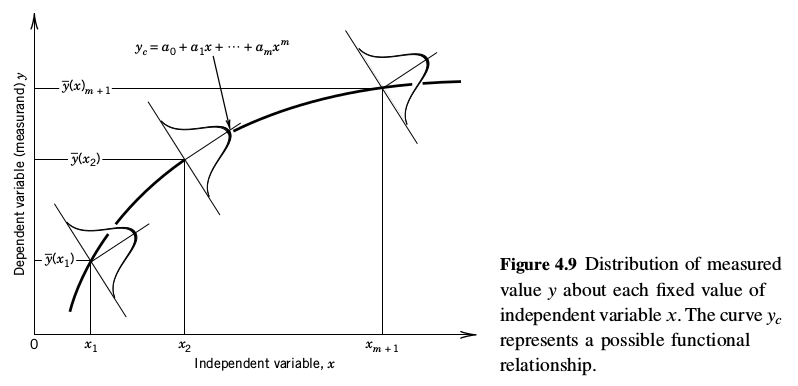
\includegraphics[scale=0.65]{lecture4_fig1.png}\\\\
 		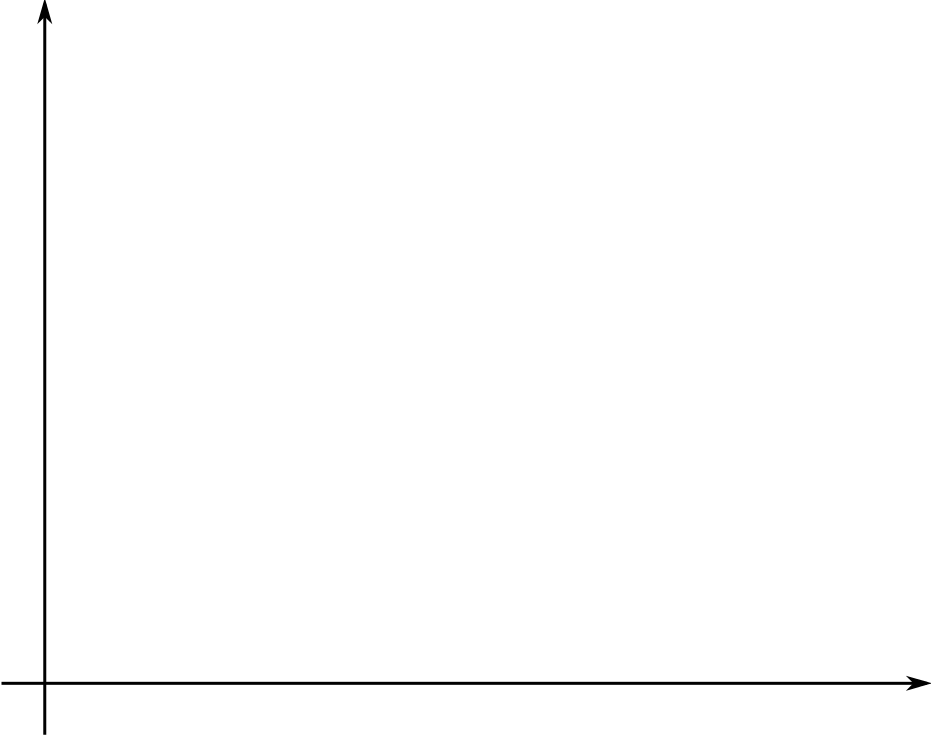
\includegraphics[scale=0.40]{lecture4_fig2.png}\\\\      
\Large
%\newpage 
\item \textbf{ \LARGE Least Squares Regression} \\\\

	\begin{itemize}
		
		\item \textbf{ We are trying to find a polynomial of best fit.}\\\\\scalebox{1.25}{$y_c(x)=a_0+a_1x+a_2x^2+\dots+a_mx^m\hspace{10mm}m\leq(n-1)$} \\\\

		\item \textbf{ This is done by minimizing the quantity below.}\\\\\scalebox{1.25}{$D=\Sigma_{i=1}^N(y_i-y_{ci})^2=\Sigma_{i=1}^N(y_i-a_0+a_1x+a_2x^2+\dots+a_mx^m)^2$} \\
\LARGE
		\item \textbf{ For a first order curve the coefficients can be solved as follows.}\\\\
		\scalebox{1.5}{$a_0=\frac{\Sigma x_i\Sigma x_i y_i-\Sigma x_i^2\Sigma y_i}{(\Sigma x_i)^2-N\Sigma x_i^2}$}
		\item \textbf{ and}\\\\
		\scalebox{1.5}{$a_1=\frac{\Sigma x_i\Sigma y_i-N\Sigma x_i y_i }{(\Sigma x_i)^2-N\Sigma x_i^2}$}



	\end{itemize}	
	\end{itemize}

\end{itemize}

	

\end{document}



